\documentclass[11pt,a4paper]{article}

\usepackage[utf8]{inputenc}
\usepackage[T1]{fontenc}
\usepackage{geometry}
\usepackage{titlesec}
\usepackage{graphicx}
\usepackage{float}
\usepackage{xcolor}
\usepackage{listings}
\usepackage{hyperref}
\usepackage{enumitem}

\geometry{margin=2.5cm}

\hypersetup{
    colorlinks=true,
    linkcolor=blue,
    urlcolor=blue
}

\titleformat{\section}
{\large\bfseries}
{\thesection.}{0.5em}{}

\titleformat{\subsection}
{\normalsize\bfseries}
{\thesubsection.}{0.5em}{}

\definecolor{codebg}{rgb}{0.95,0.95,0.95}

\lstset{
    backgroundcolor=\color{codebg},
    basicstyle=\ttfamily\small,
    frame=single,
    breaklines=true,
    columns=fullflexible
}

\begin{document}

\begin{titlepage}
    \centering

    \vspace*{3cm}

    {\Huge \textbf{LAMP Stack Deployment and SELinux Configuration}}\\[1cm]

    {\Large Server Engineering Labs}\\[2cm]

    \textbf{Author:}\\
    Laura Ortiz Moreno\\[1cm]

    \textbf{Topics Covered:}
    \begin{itemize}[leftmargin=4cm]
        \item Apache HTTP Server
        \item MariaDB database server
        \item PHP integration
        \item Linux service management
        \item SELinux configuration
        \item Web application deployment
    \end{itemize}

    \vfill

    \textbf{Environment:}\\
    Debian Linux Server\\
    Rocky Linux Client VM\\
    Virtualized lab environment

    \vspace{1cm}

\end{titlepage}

\tableofcontents
\newpage

\section{Introduction}

This report documents the deployment and validation of a LAMP environment in Linux.

The laboratory focused on:
\begin{itemize}
    \item Installing Apache, MariaDB, and PHP
    \item Configuring system services
    \item Deploying a basic web application
    \item Verifying database connectivity
    \item Troubleshooting SELinux-related access restrictions
\end{itemize}

The setup was performed in a virtualized client-server environment using Linux virtual machines.

\section{Installing Apache Web Server}

The Apache HTTP server was installed using the Debian package manager.

Installation command:

\begin{lstlisting}[language=bash]
sudo apt update
sudo apt install apache2
\end{lstlisting}

The service status was verified:

\begin{lstlisting}[language=bash]
sudo systemctl status apache2
\end{lstlisting}

Apache was configured to start automatically on boot:

\begin{lstlisting}[language=bash]
sudo systemctl enable apache2
\end{lstlisting}

\subsection{Verification}

The server was tested from a client machine using a web browser.

Successful deployment was confirmed when the Apache default page became accessible.

\section{Installing MariaDB}

MariaDB was installed to provide relational database support.

Installation:

\begin{lstlisting}[language=bash]
sudo apt install mariadb-server
\end{lstlisting}

The service was started and enabled:

\begin{lstlisting}[language=bash]
sudo systemctl enable mariadb
sudo systemctl start mariadb
\end{lstlisting}

Verification:

\begin{lstlisting}[language=bash]
sudo systemctl status mariadb
\end{lstlisting}

\subsection{Basic Database Security}

The database server was secured using:

\begin{lstlisting}[language=bash]
sudo mysql_secure_installation
\end{lstlisting}

Typical configuration tasks included:
\begin{itemize}
    \item Removing anonymous users
    \item Disabling remote root login
    \item Removing test databases
    \item Enforcing secure credentials
\end{itemize}

\section{Installing PHP}

PHP support was installed to allow dynamic content generation.

Packages installed:

\begin{lstlisting}[language=bash]
sudo apt install php libapache2-mod-php php-mysql
\end{lstlisting}

The Apache service was restarted:

\begin{lstlisting}[language=bash]
sudo systemctl restart apache2
\end{lstlisting}

\subsection{PHP Validation}

A test file was created inside the Apache web root:

\begin{lstlisting}[language=bash]
sudo nano /var/www/html/info.php
\end{lstlisting}

Content:

\begin{lstlisting}[language=PHP]
<?php
phpinfo();
?>
\end{lstlisting}

The page was then accessed from the browser to verify PHP integration.

\section{Database Connectivity Testing}

A simple database connection test was performed using PHP.

Example:

\begin{lstlisting}[language=PHP]
<?php
$conn = new mysqli("localhost", "user", "password", "database");

if ($conn->connect_error) {
    die("Connection failed");
}

echo "Database connection successful";
?>
\end{lstlisting}

The objective was to verify:
\begin{itemize}
    \item PHP-MariaDB integration
    \item Database service accessibility
    \item Web application functionality
\end{itemize}

\begin{figure}[H]
    \centering
    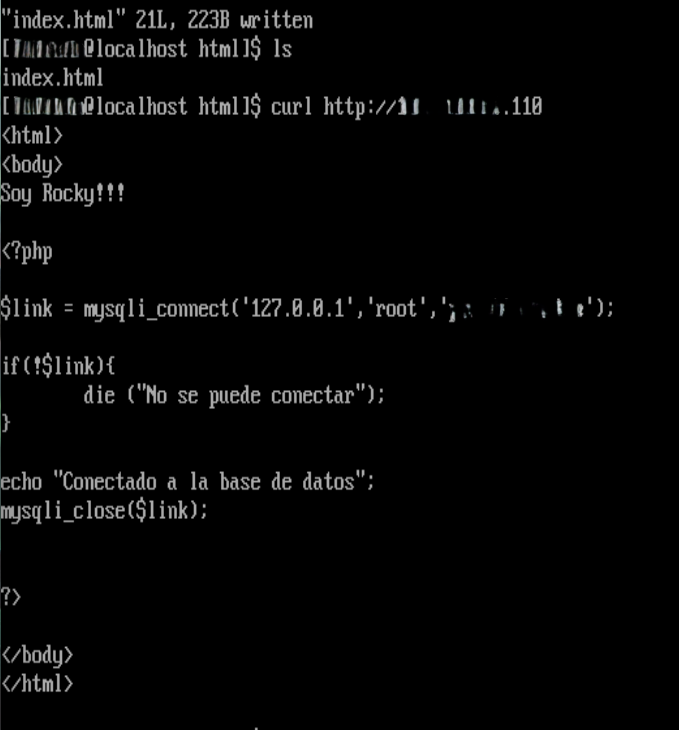
\includegraphics[width=0.82\textwidth]{images/lamp/php-db-test.png}
    \caption{Validation of Apache, PHP, and MariaDB integration using a simple PHP database connection test.}
\end{figure}

\section{SELinux Configuration and Troubleshooting}

Part of the laboratory focused on understanding how SELinux affects services and filesystem access.

Useful commands included:

\begin{lstlisting}[language=bash]
getenforce
sestatus
\end{lstlisting}

SELinux contexts were inspected using:

\begin{lstlisting}[language=bash]
ls -Z
\end{lstlisting}

When required, contexts were restored using:

\begin{lstlisting}[language=bash]
restorecon -Rv /var/www/html
\end{lstlisting}

\subsection{SELinux Boolean Configuration}

SELinux booleans were modified to allow Apache to communicate with the database service.

\begin{lstlisting}[language=bash]
sudo setsebool -P httpd_can_network_connect_db on
\end{lstlisting}

The configuration was validated using:

\begin{lstlisting}[language=bash]
sudo getsebool -a | grep httpd_can_network
\end{lstlisting}

\begin{figure}[H]
    \centering
    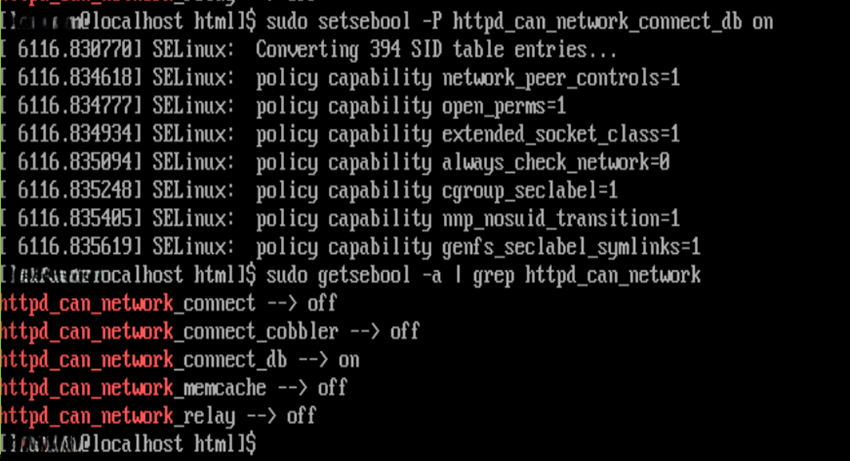
\includegraphics[width=0.86\textwidth]{images/lamp/selinux-db-boolean.png}
    \caption{SELinux boolean configuration allowing Apache HTTP services to connect to the database backend.}
\end{figure}

\subsection{Firewall Verification}

Firewall rules were also validated to ensure HTTP traffic was allowed.

Example:

\begin{lstlisting}[language=bash]
sudo ufw allow 80/tcp
sudo ufw reload
\end{lstlisting}

\section{Service Validation}

The environment was tested from external clients to validate:
\begin{itemize}
    \item Apache availability
    \item PHP execution
    \item Database connectivity
    \item Firewall accessibility
\end{itemize}

The complete LAMP stack operated correctly after service configuration and troubleshooting.

\section{Challenges Encountered}

Several issues appeared during deployment:
\begin{itemize}
    \item Apache service conflicts
    \item PHP module configuration errors
    \item Database permission problems
    \item SELinux access denials
    \item Firewall restrictions
\end{itemize}

The exercises provided practical troubleshooting experience in Linux server administration.

\section{Conclusion}

This laboratory introduced the deployment and administration of a complete LAMP environment.

The exercises demonstrated:
\begin{itemize}
    \item Linux web server deployment
    \item Database administration basics
    \item PHP integration
    \item SELinux troubleshooting
    \item Service validation and monitoring
\end{itemize}

These concepts are essential in backend infrastructure, Linux administration, and web server management.

\end{document}